\documentclass{beamer}
%
% Choose how your presentation looks.
%
% For more themes, color themes and font themes, see:
% http://deic.uab.es/~iblanes/beamer_gallery/index_by_theme.html
%
\mode<presentation>
{
  \usetheme{default}      % or try Darmstadt, Madrid, Warsaw, ...
  \usecolortheme{default} % or try albatross, beaver, crane, ...
  \usefonttheme{default}  % or try serif, structurebold, ...
  \setbeamertemplate{navigation symbols}{}
  \setbeamertemplate{caption}[numbered]
} 

\usepackage[english]{babel}
\usepackage[utf8x]{inputenc}
\usepackage[style=british]{csquotes}
\def\signed #1{{\leavevmode\unskip\nobreak\hfil\penalty50\hskip1em
		\hbox{}\nobreak\hfill #1%
		\parfillskip=0pt \finalhyphendemerits=0 \endgraf}}
\usepackage{mathptmx}
\usepackage[T1]{fontenc}
\usepackage{amsmath}
\usepackage{amssymb}
\usepackage{graphicx}
\usepackage{sansmathaccent}
\usepackage{hyperref}
\pdfmapfile{+sansmathaccent.map}
\newsavebox\mybox
\newenvironment{aquote}[1]
{\savebox\mybox{#1}\begin{quote}}
	{\vspace*{1mm}\signed{\usebox\mybox}\end{quote}}

\AtBeginSection[]{
	\begin{frame}
	\vfill
	\centering
	\begin{beamercolorbox}[sep=8pt,center,shadow=true,rounded=true]{title}
		\usebeamerfont{title}\secname\par%
	\end{beamercolorbox}
	\vfill
\end{frame}
}



\title[Your Short Title]{Convergence and Divergence\\ in European Bond Correlations}
\author{Peter Schwendner, Martin Schüle and Martin Hillebrand}
\institute{Zurich University of Applied Sciences}
\date{16.10.2019}

\newcommand{\avg}[1]{\left< #1 \right>} % for average

\begin{document}

\begin{frame}
  \titlepage
\end{frame}

% Uncomment these lines for an automatically generated outline.
%\begin{frame}{Outline}
%  \tableofcontents
%\end{frame}



\begin{frame}{European Bond Yields (daily Bloomberg data)}
\begin{itemize}
	\item Euro convergence for bonds yields during end of 90s.
	\item Wide spreads during European sovereign debt crisis 2010-2012.
	\item Since 2015, bond spreads primarily signal political divergence. 
\end{itemize}

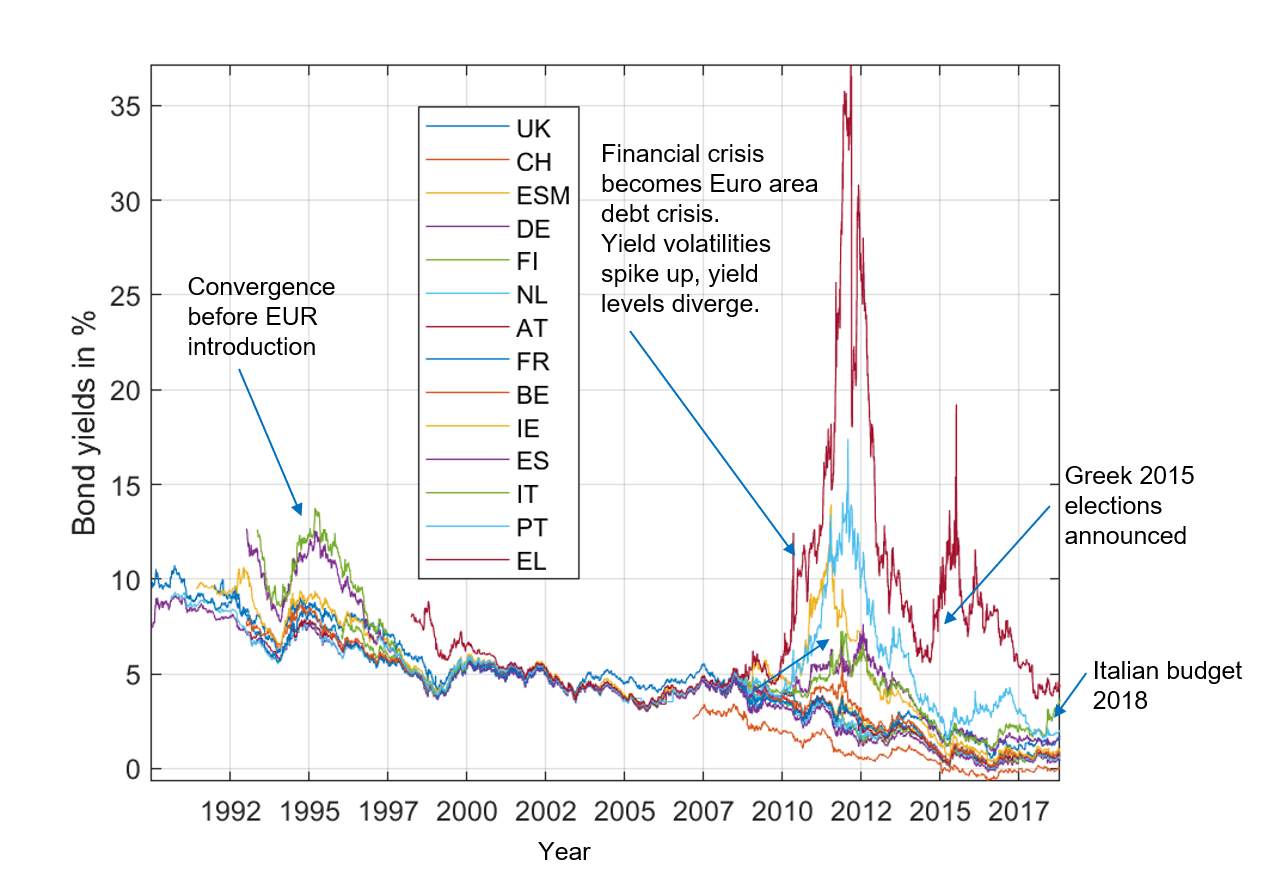
\includegraphics[height=7cm]{yields}.

\end{frame}






\begin{frame}{European Bond Return Correlations 2008 - 2013}
\begin{itemize}
\item Containment of the 2010 sovereign bond crisis
\end{itemize}

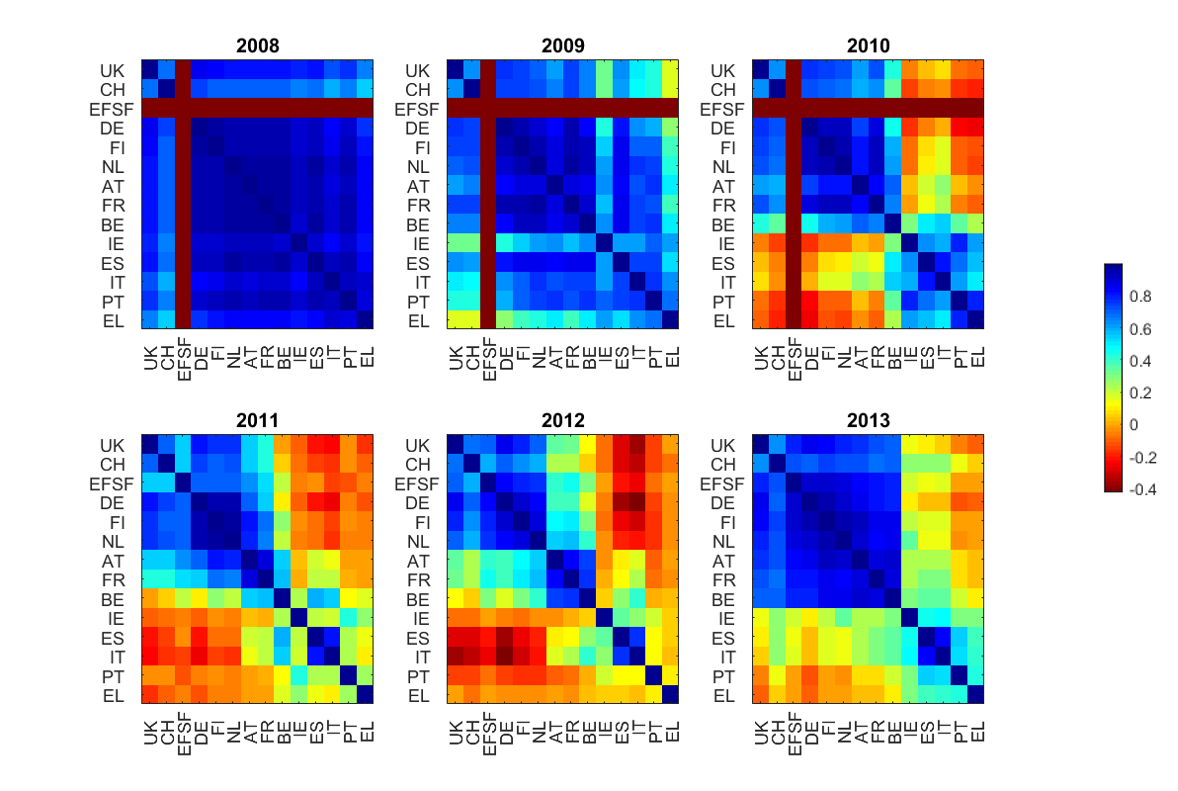
\includegraphics[height=7cm]{2008-2013}

%\includegraphics[height=\baselineskip]{example-image}.

%\includegraphics[height=3cm]{example-image-a}\includegraphics[width=5cm]{example-image-b}

%\includegraphics[height=3cm]{example-image-a} \includegraphics[width=5cm]{example-image-b}

\end{frame}


\begin{frame}{European Bond Return Correlations 2014-2019}
\begin{itemize}
\item From financial crisis to political divergence 
\end{itemize}

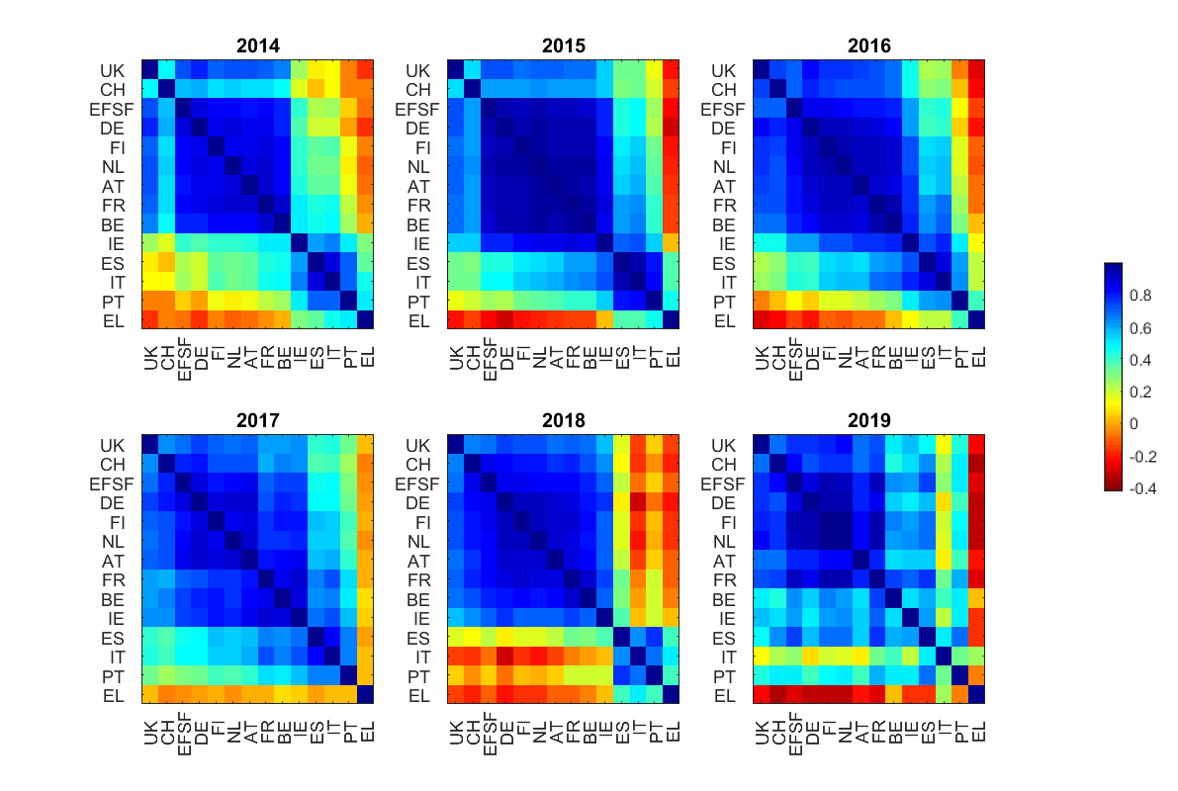
\includegraphics[height=7cm]{2014-2019}

%\includegraphics[height=\baselineskip]{example-image}.

%\includegraphics[height=3cm]{example-image-a}\includegraphics[width=5cm]{example-image-b}

%\includegraphics[height=3cm]{example-image-a} \includegraphics[width=5cm]{example-image-b}
\end{frame}

\begin{frame}{Problems with correlations}
\begin{itemize}
  \item They are unstable in time
 \item Common factors may lead to spurious correlations
 \item Too many links: each market is correlated to any other market. Who is driving what?
 \item Idea: "Correlation influence" shows driving factors of correlations.
Bootstrap resampling to simulate statistical noise in return blocks of random length ("wild bootstrap").
\end{itemize}
\includegraphics[width=10cm]{bootstrap_resampling.pdf}

\end{frame}





\begin{frame}{Correlation influence Network}
\begin{itemize}
  \item The partial correlation measure is defined as
 \begin{eqnarray}
\rho_{ij:k} = \frac{C_{ij} - C_{ik}C_{kj}}{\sqrt{1-C_{ik}^2} \sqrt{1-C_{kj}^2}}.
\label{partial_correlation}
\end{eqnarray}

  \item  Correlation influence is defined as
\begin{eqnarray}
d_{i,j:k}=C_{ij}-\rho_{ij:k}.
\end{eqnarray}

\item The average correlation influence is defined as
\begin{eqnarray}
d_{i:k}=\avg{d_{i,j:k}}_{j \neq i,k}.
\label{d_ik}
\end{eqnarray}
This is a directed arrow from market $k$ pointing to market $i$.
\end{itemize}

Ref.: Kenett D. Y. et. al.: Dominating clasp of the financial sector revealed by partial correlation analysis of the stock market. PLoS ONE 5(12): e15032. 

\end{frame}


\begin{frame}{Bootstrap filter}
\begin{itemize}
\item For each resample, we compute the average correlation influence matrix.  
\item The standard deviation across all resamples is a measure for the noise in the correlation influence.
\item We filter out correlation influences with a threshold of three standard deviations.

\end{itemize}


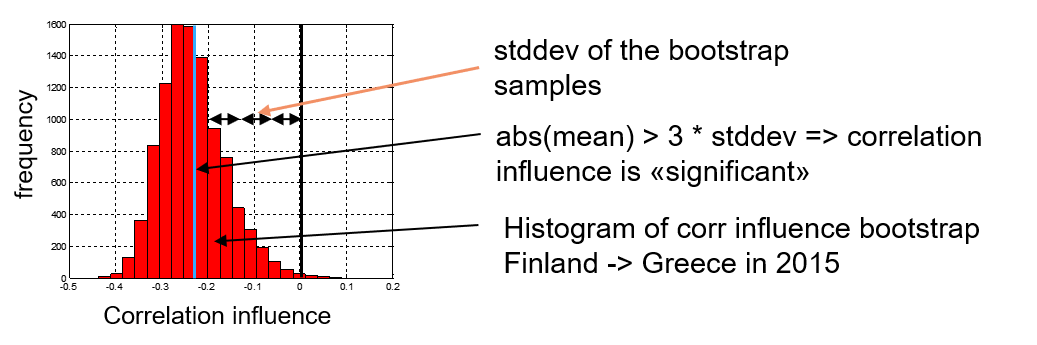
\includegraphics[width=12cm]{bootstrap}

\end{frame}



\begin{frame}{Overview: Generate Filtered Correlation Influence Network}

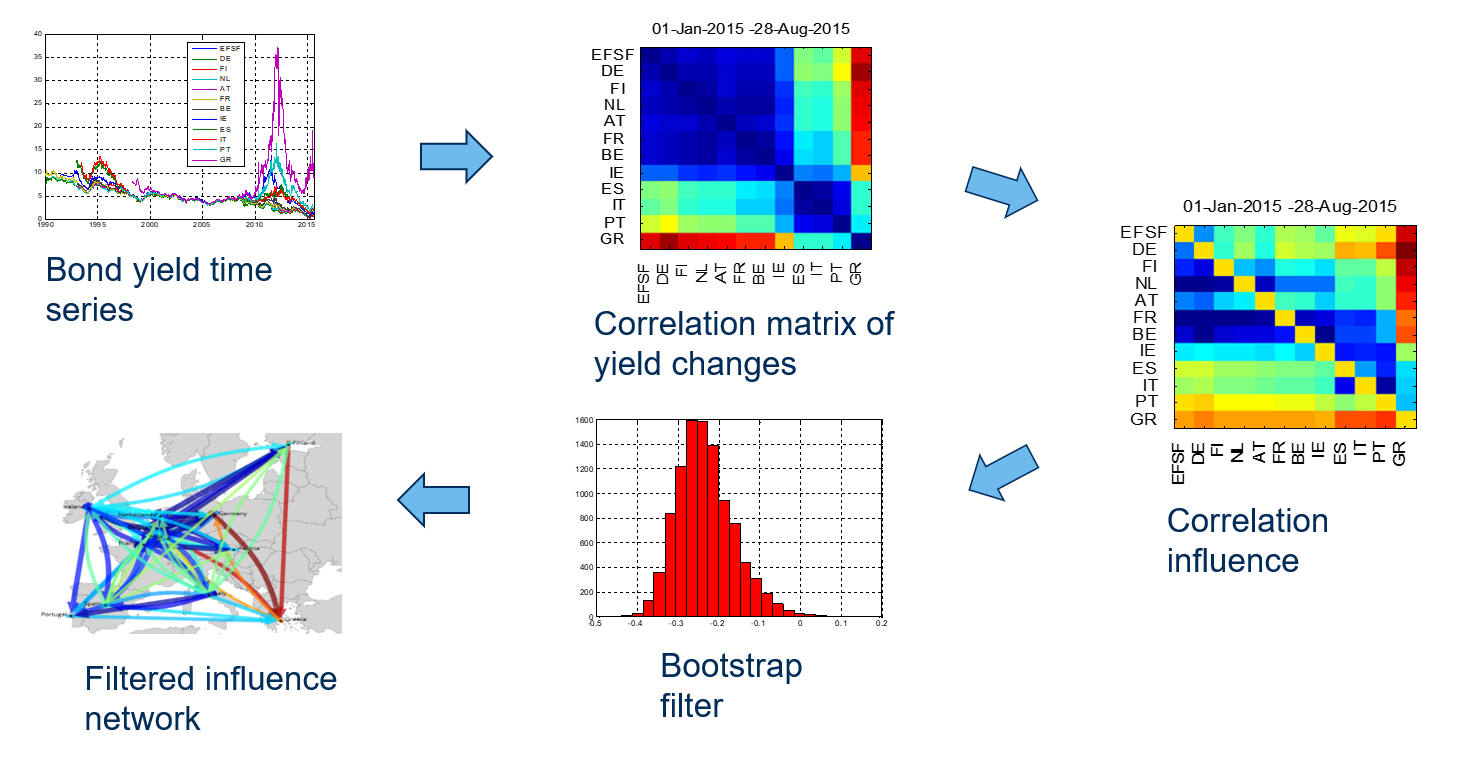
\includegraphics[height=6cm]{scheme}
Positive correlation influences: {\color{blue} blue arrows}\\ 
Negative correlation influences: {\color{red} red arrows}

\end{frame}


\begin{frame}{Filtered Correlation Influence Networks 2008 - 2013}
\vspace{-0.0cm}\hspace*{-1cm}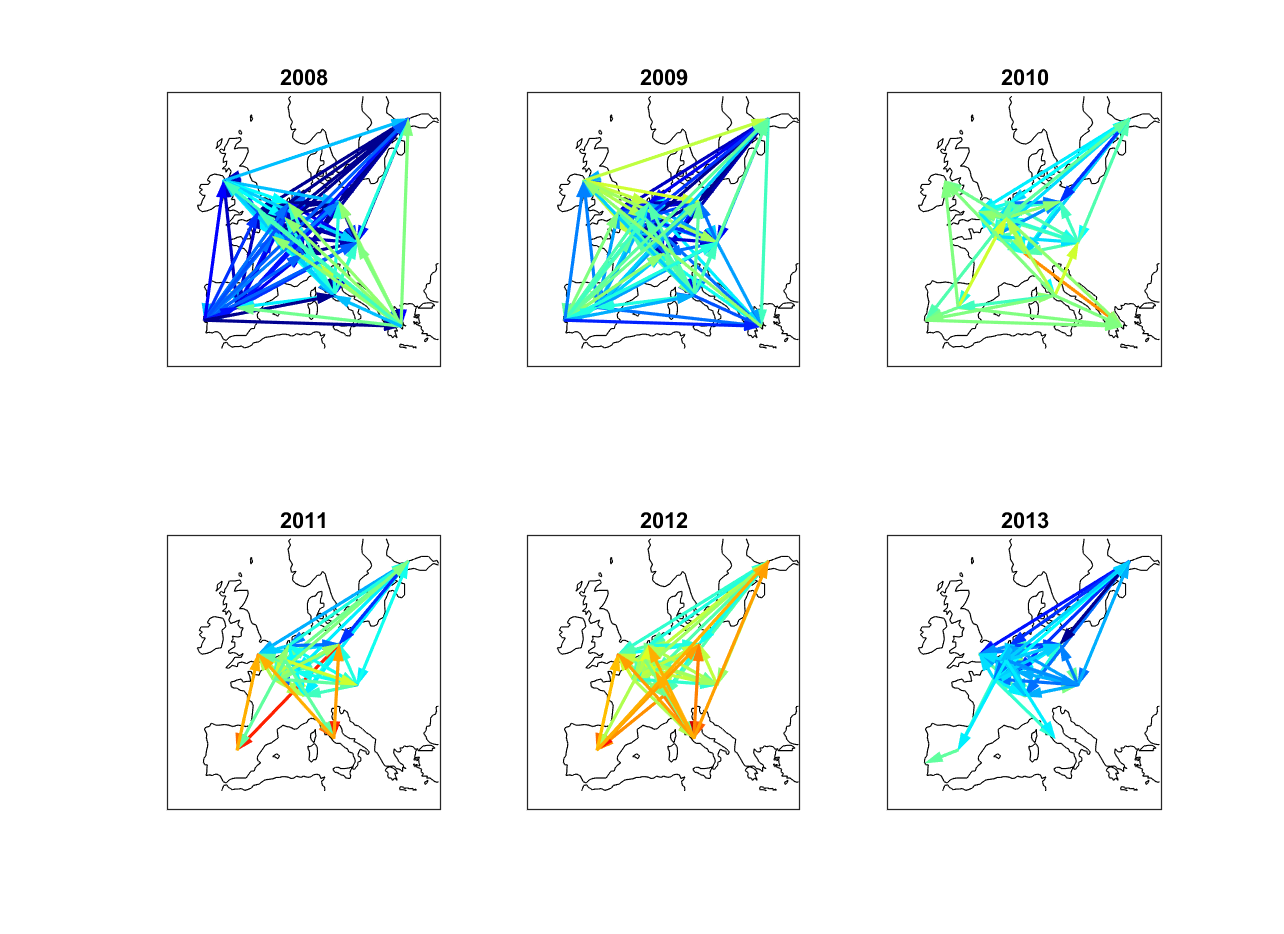
\includegraphics[height=9cm]{networks2008-2013}
%\includegraphics[height=\baselineskip]{example-image}.

%\includegraphics[height=3cm]{example-image-a}\includegraphics[width=5cm]{example-image-b}

%\includegraphics[height=3cm]{example-image-a} \includegraphics[width=5cm]{example-image-b}

\end{frame}




\begin{frame}{Filtered Correlation Influence Networks 2014 - 2019}
\vspace{-0.0cm}\hspace*{-1cm}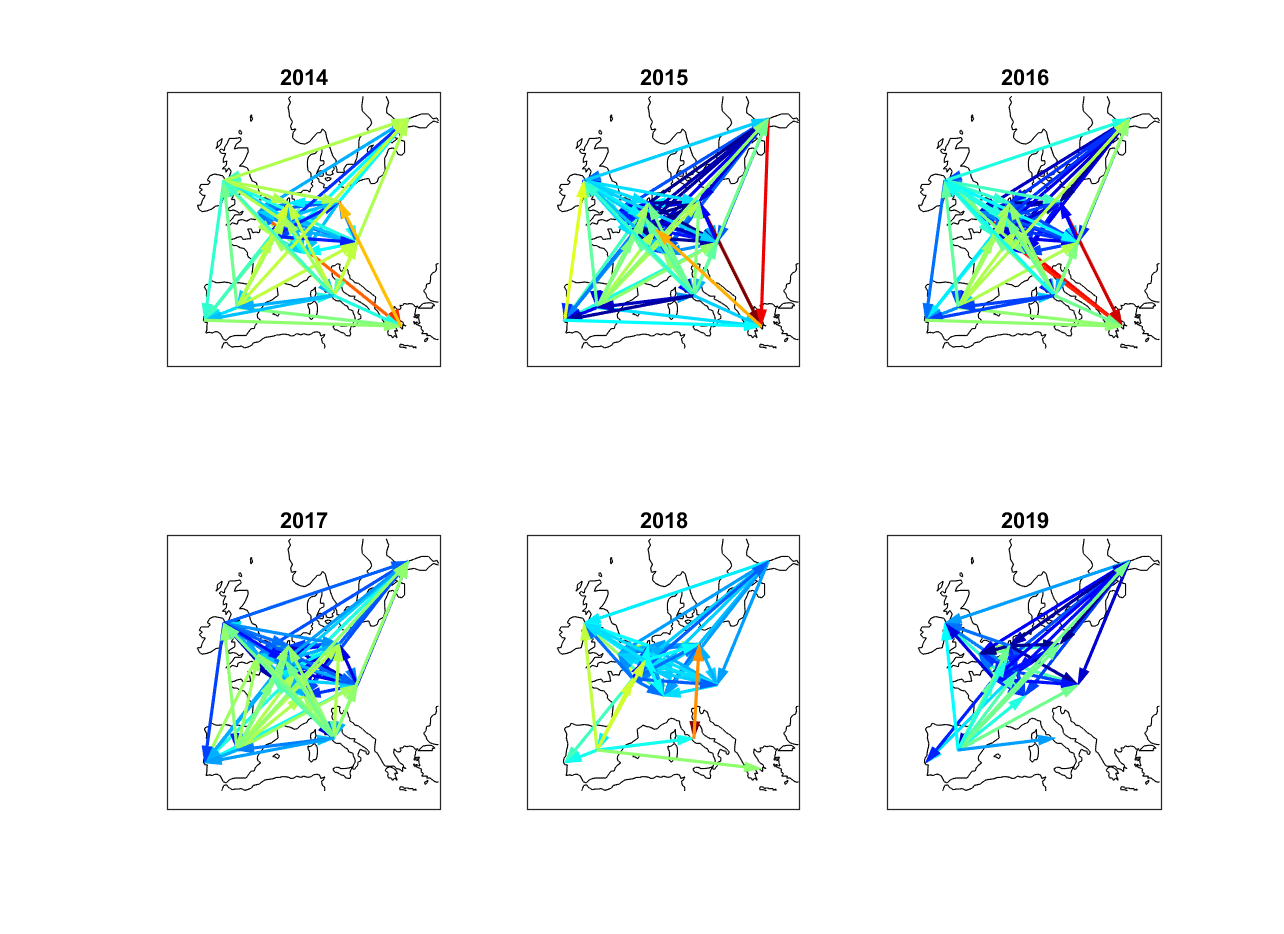
\includegraphics[height=9cm]{networks2014-2019}
%\includegraphics[height=\baselineskip]{example-image}.

%\includegraphics[height=3cm]{example-image-a}\includegraphics[width=5cm]{example-image-b}

%\includegraphics[height=3cm]{example-image-a} \includegraphics[width=5cm]{example-image-b}

\end{frame}


\begin{frame}{Filtered Correlation Influence Networks October 2018}
\vspace{-0.0cm}\hspace*{-1cm}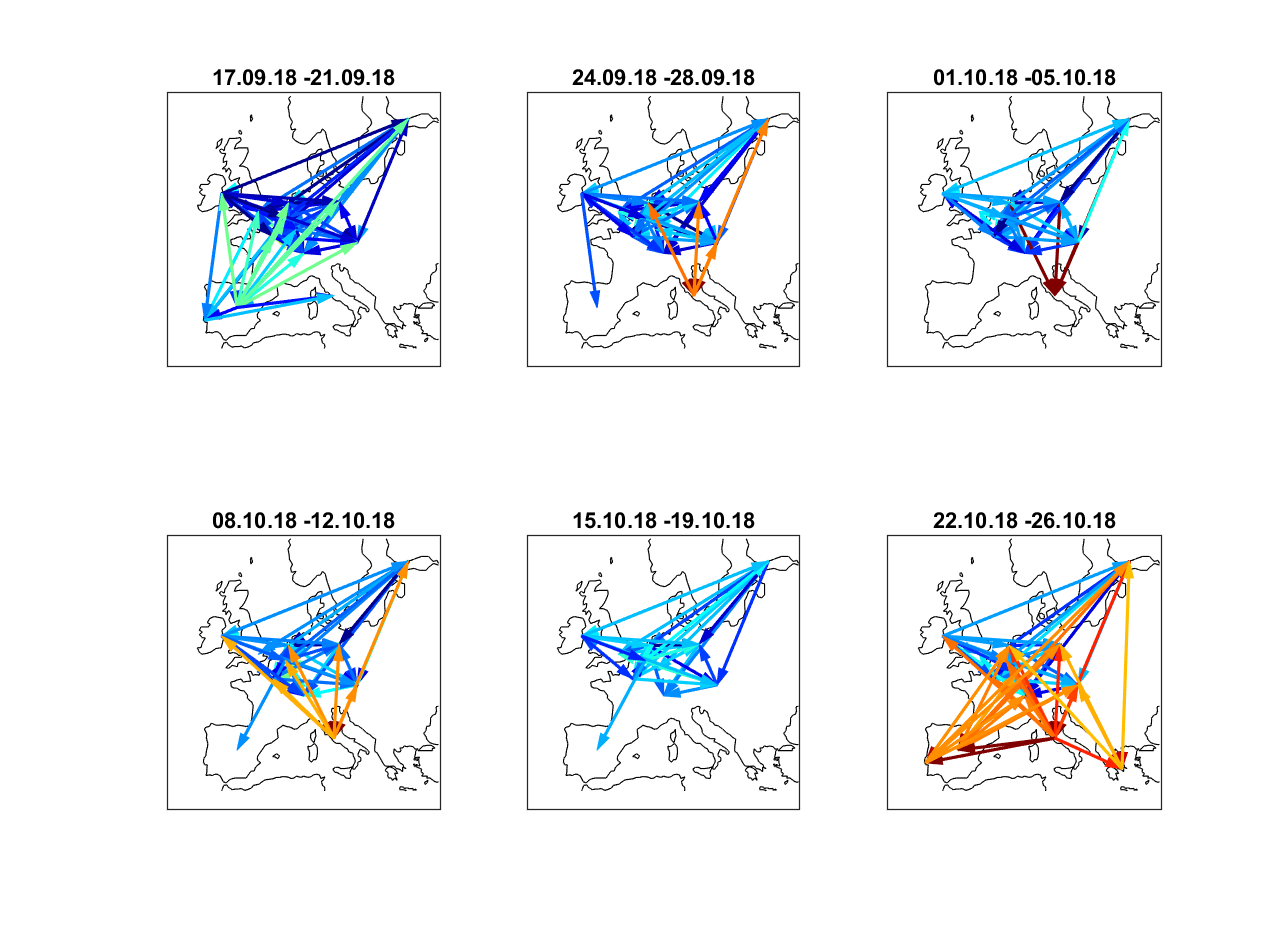
\includegraphics[height=9cm]{networks26-10-2018}
%\includegraphics[height=\baselineskip]{example-image}.

%\includegraphics[height=3cm]{example-image-a}\includegraphics[width=5cm]{example-image-b}

%\includegraphics[height=3cm]{example-image-a} \includegraphics[width=5cm]{example-image-b}
\end{frame}

\begin{frame}{Filtered Correlation Influence Networks August 2019}
\vspace{-0.00cm}\hspace*{-1cm}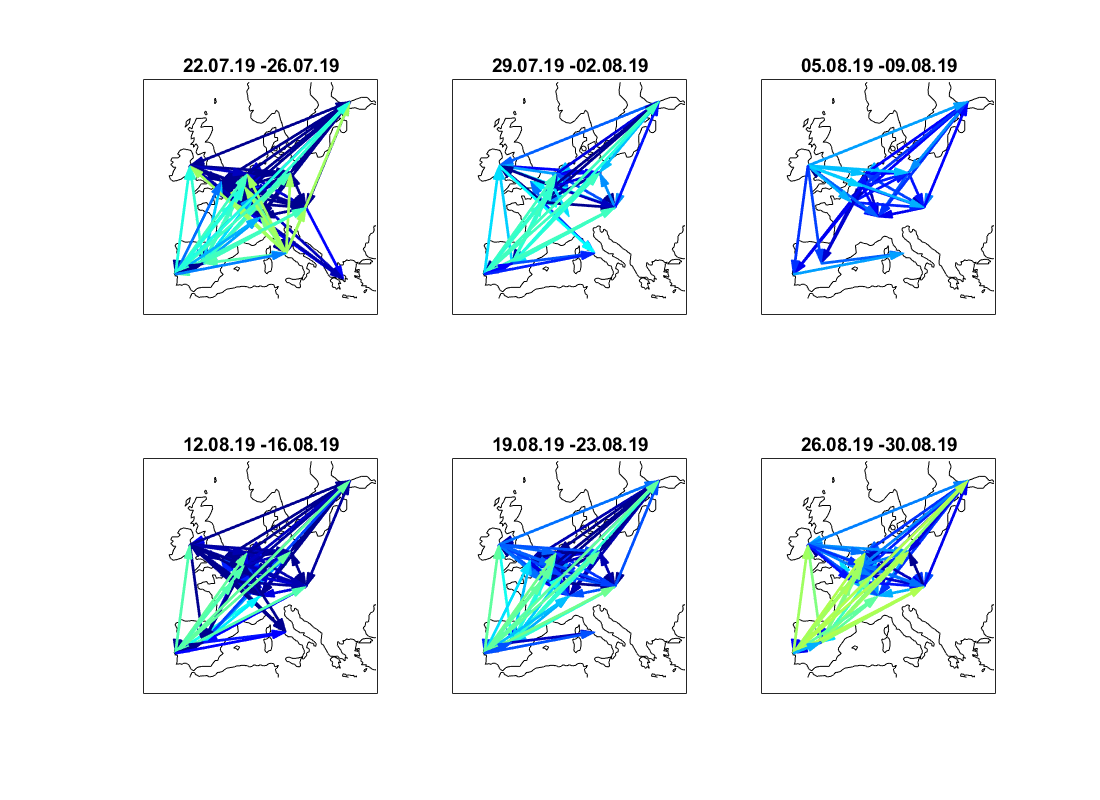
\includegraphics[height=9cm]{networks30-08-2019}
%\includegraphics[height=\baselineskip]{example-image}.

%\includegraphics[height=3cm]{example-image-a}\includegraphics[width=5cm]{example-image-b}

%\includegraphics[height=3cm]{example-image-a} \includegraphics[width=5cm]{example-image-b}
\end{frame}





\begin{frame}{Publicly available European Bond Yield data}
\begin{itemize}
	\item Source: ECB https://sdw.ecb.europa.eu
	\item Only monthly, but 27 EU countries (all but Estonia)
\end{itemize}
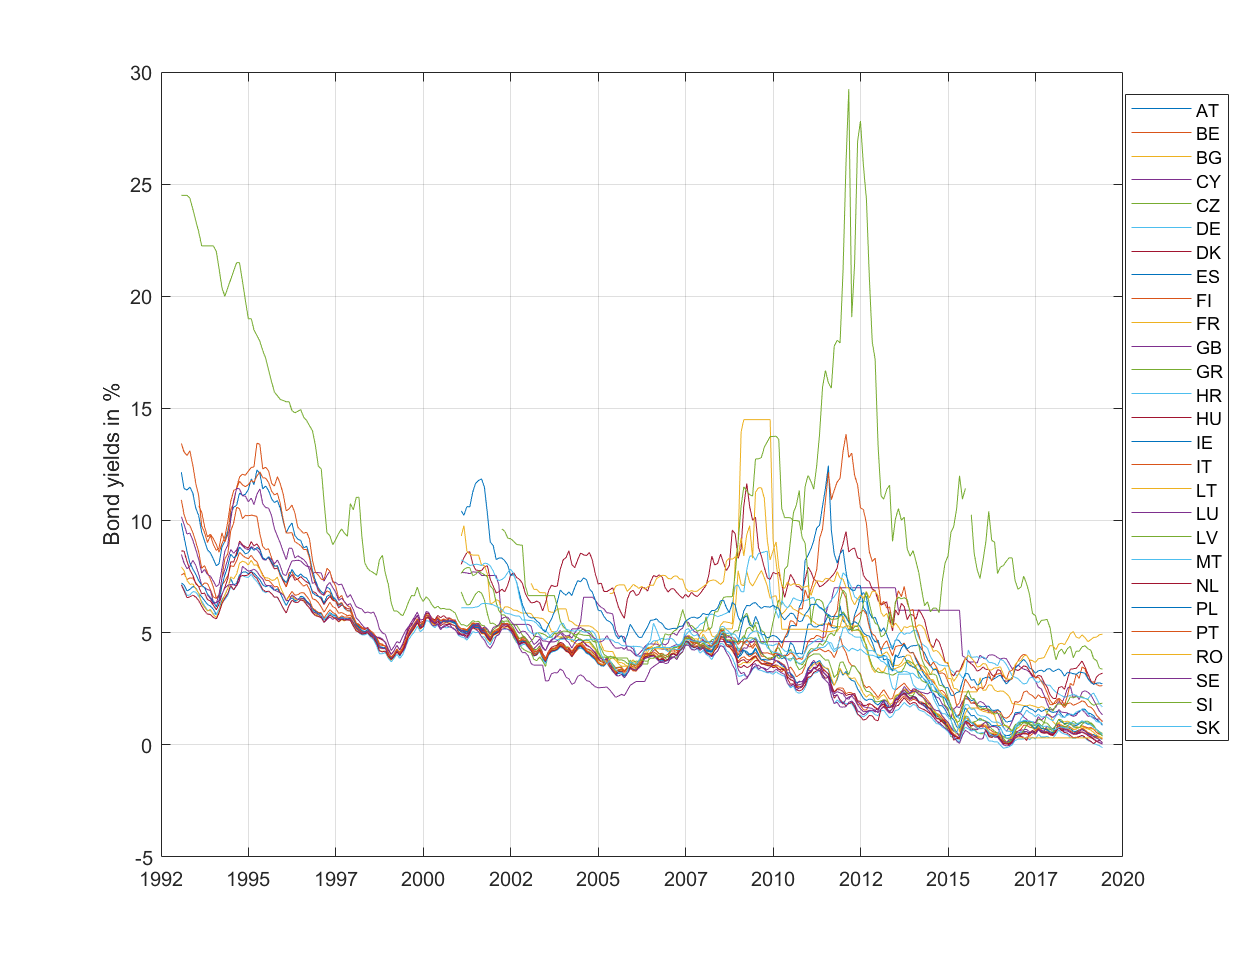
\includegraphics[height=7cm]{yields-monthly}.

\end{frame}


\begin{frame}{European Bond Return Correlations 2002 - 2019}
\begin{itemize}
\item We define 3-year-windows as we only have monthly data
\end{itemize}

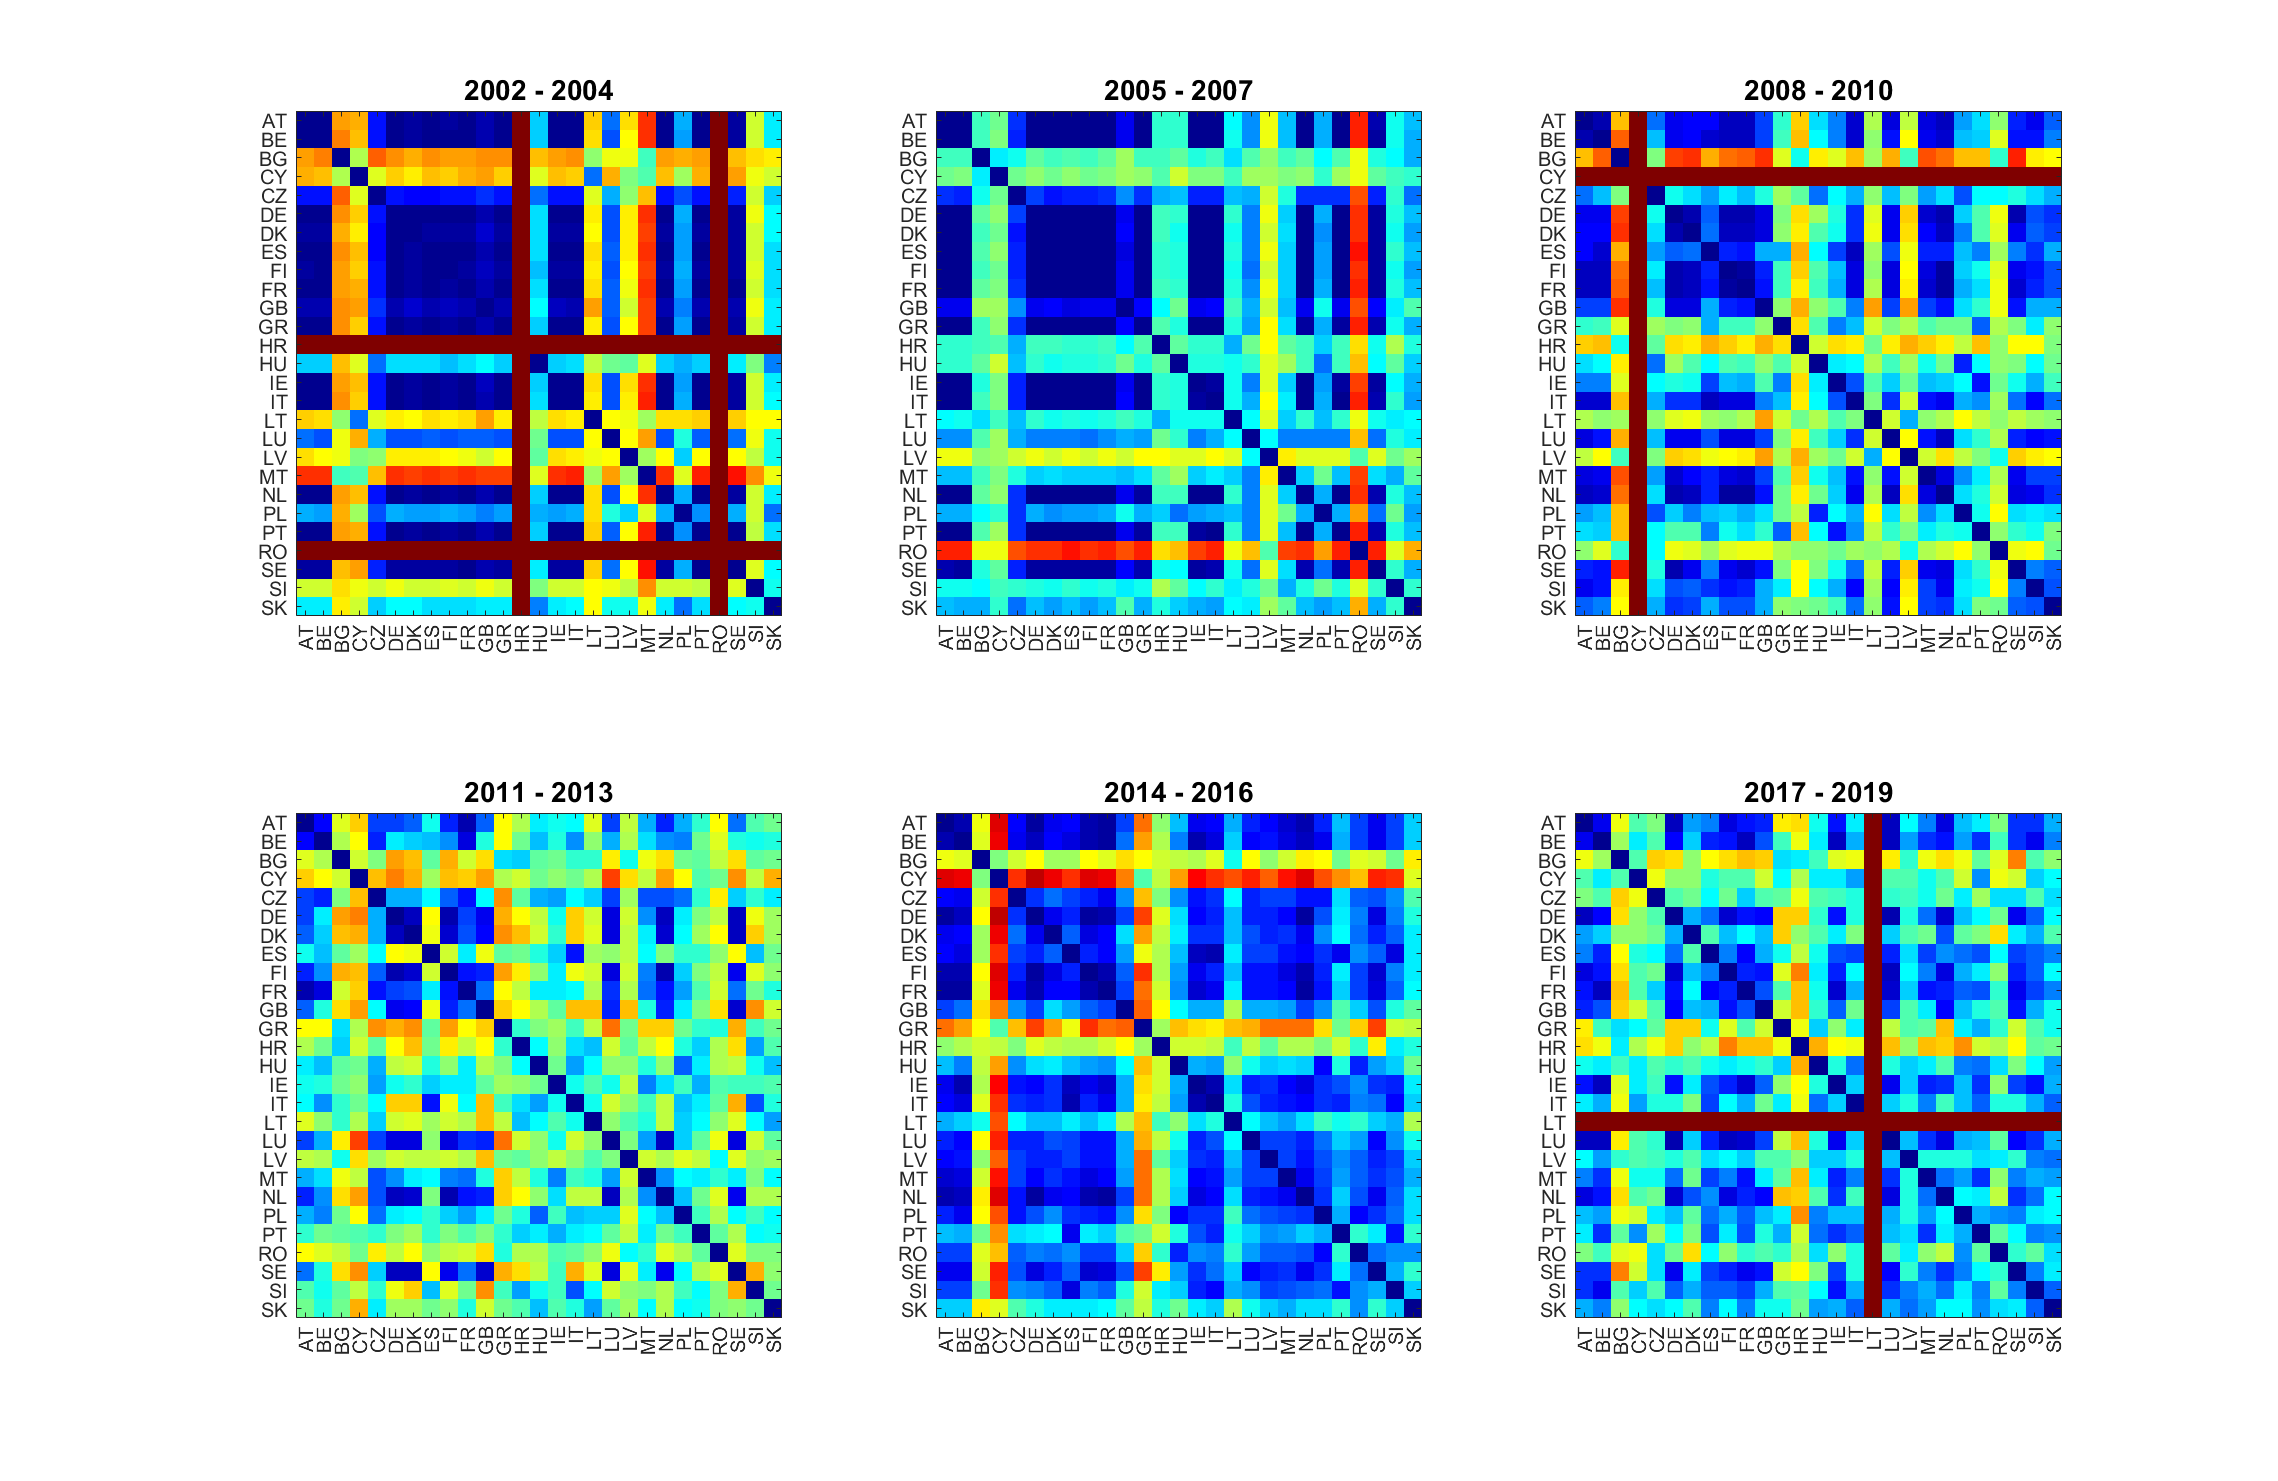
\includegraphics[height=7cm]{heatmaps-monthly}

\end{frame}


\begin{frame}{Filtered Correlation Influence Networks 2002 - 2019}
\begin{itemize}
\item Also with monthly data, the networks replicate the core-periphery dynamics
\end{itemize}
\vspace{0cm}\hspace*{-1cm}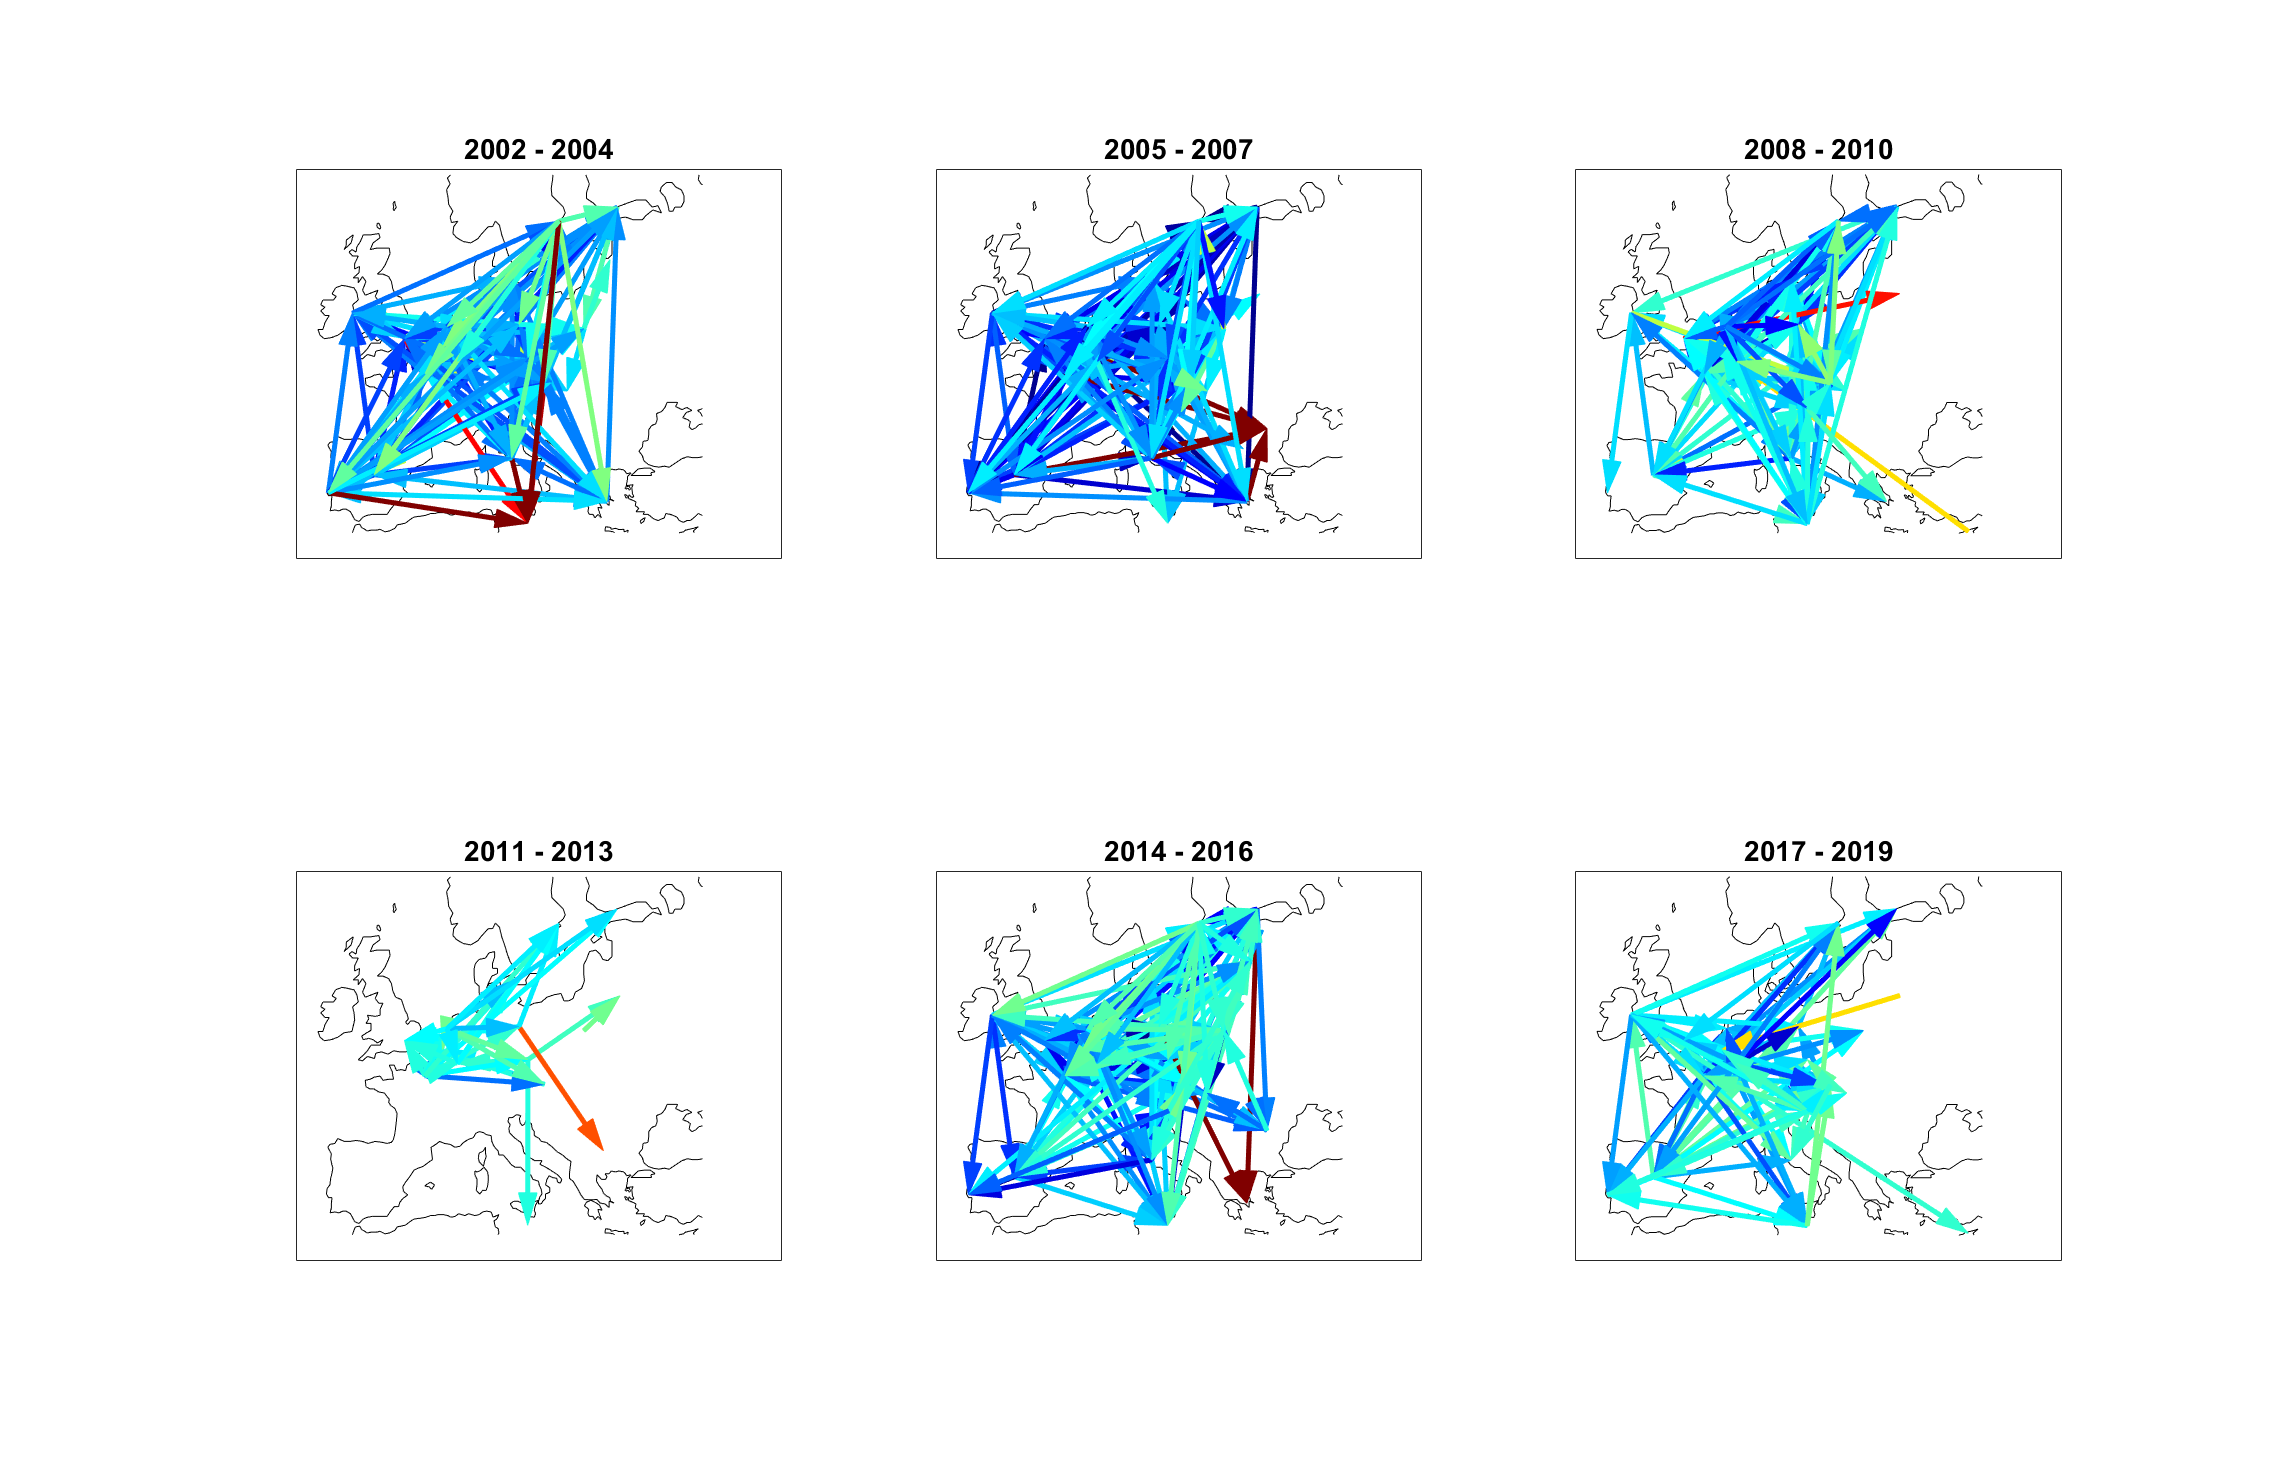
\includegraphics[height=8cm]{networks-monthly}
\end{frame}




\begin{frame}{Conclusions}
\begin{itemize}
\item Since 2010, European bonds cluster into core and periphery groups according to their return correlations. We use filtered correlation influence networks to show the most significant drivers of convergence and divergence.
\item During the European sovereign debt crisis 2010 - 2012, negative correlation influences between the core and periphery groups are the dominating force. Since 2013, the situation improved a lot.
\item In 2015 during the negotiations between Greece and the Eurogroup and in 2018 during the Italian budget negotiations, the warning signals of negative correlation influences reappeared for short periods, although the absolute level of spreads is substantially smaller than during 2010 - 2012.
\item The findings point to markets becoming more politically driven.
\end{itemize}
Full papers: \href{https://www.esm.europa.eu/publications/european-government-bond-dynamics-and-stability-policies-taming-contagion-risks}{ESM Working Paper \#8 and JNTF (2015)}, \href{https://www.frontiersin.org/articles/10.3389/frai.2019.00020/full}{"Sentiment Analysis of European Bonds 2016 - 2018" , Frontiers in AI (2019)}.
\end{frame}


\end{document}